\documentclass{article}
\usepackage{amsmath}
\usepackage{tikz}
\begin{document}

\title{Geometry in high dimensions}
\author{}
\date{\vspace{-10ex}}
\maketitle


\section{Close-packing fraction}

We first compute the close packing fraction
in a high dimension,
which is the fraction of packing equal hyperspheres
in a high-dimensional close-packing lattice analogous to
the triangular and faced-centered cubic (FCC) lattices.
%
Our calculation consists of three steps.

\begin{enumerate}
\item
The volume of the unit cell of a $D$-dimensional
close-packing lattice is given by
\begin{equation}
  U_D
  =
  \sqrt{ \frac{ D + 1 }
              {  2^D  } }.
  \label{eq:vunitcell}
\end{equation}

\item
The volume of the $D$-dimensional hypersphere
of unit diameter is given by
\begin{equation}
  V^{1/2}_D
  =
  \frac{     { \sqrt \pi }^D      }
       {  \Gamma(\frac D 2 + 1 )  }
  \left( \frac{ 1 } { 2 } \right)^D
  .
  \label{eq:vsphrhalf}
\end{equation}

\item
Therefore, the close packing fraction is given by
\begin{equation}
  \eta^\mathrm{cp}_D
  =
  \frac{ V_D^{1/2} }
       { U_D       }
  =
  \frac{ \sqrt{ \pi / 2 }^D }
       { \sqrt{ D + 1 } \,
         \Gamma\left( \frac D 2 + 1 \right) }
  .
  \label{eq:packfrac}
\end{equation}

\end{enumerate}

Below, we give details leading to the first two steps. 
%
Note that Eq. \eqref{eq:vsphrhalf} is useful by itself,
as the packing fraction $\eta_D$
of any $D$-dimensional structure is defined as
$$
\eta_D = V^{1/2}_D \, \rho_D,
$$
where $\rho_D$ is the number density.



\section{Volume of the unit cell in a close-packing lattice}

To show Eq. \eqref{eq:vunitcell}, we argue that

\begin{enumerate}
\item
A $D$-dimensional close-packing lattice
consists of layers of $(D-1)$-dimensional
close-packing lattices.

\item
The $(D-1)$-dimensional layers are stacked
in such a way that the vertices of neighboring layers
form regular $D$-dimensional tetrahedra of unit sides.

\item
In the tetrahedron,
let the distance from a vertex to the opposite face
be $h_D$,
which is also the distance between two neighboring layers.
%
Then, by computing the coordinates of the center of mass
(see Fig. \ref{fig:vunitcell}),
we get the distance between a vertex to
the center of the tetrahedron,
%
\begin{equation}
  r_D
  =
  \frac{   D   }
       { D + 1 }
  h_D.
  \label{eq:rD_hD}
\end{equation}


\begin{figure}[h]
\centering
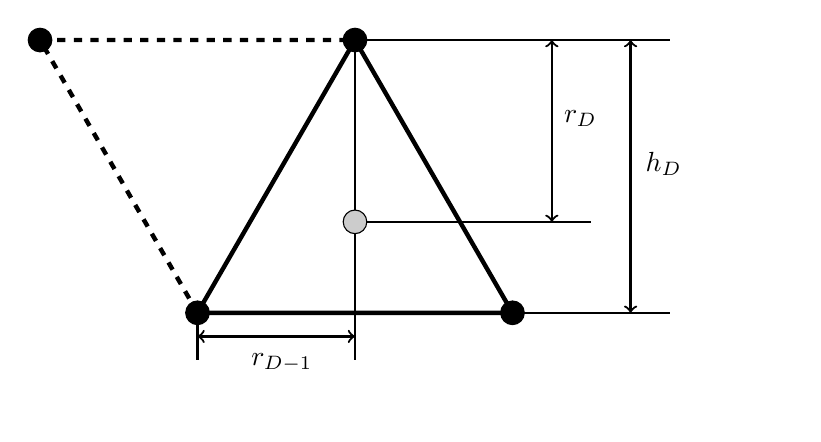
\begin{tikzpicture}
\draw[ultra thick] (-2.0, 0) -- (2.0, 0) -- (0.0, 3.464) -- cycle;
\draw[ultra thick, dashed]
   (-2.0, 0) -- (-4.0, 3.464) -- (0.0, 3.464);
\draw[thick] (-2.0, 0)     -- (-2.0, -0.6)
             ( 0.0, 3.464) -- ( 0.0, -0.6);
\draw[thick, <->] (-2.0, -0.3) -- (0.0, -0.3)
    node[anchor=20, inner sep=15] {$r_{D - 1}$};
\draw[thick] ( 0.0, 3.464) -- ( 4.0, 3.464)
             ( 0.0, 1.155) -- ( 3.0, 1.155)
             ( 2.0, 0.0)   -- ( 4.0, 0.0);
\draw[thick, <->] (2.5, 1.155) -- (2.5, 3.464)
    node[anchor=110, inner sep=25] {$r_D$};
\draw[thick, <->] (3.5, 0.0)   -- (3.5, 3.464)
    node[anchor=105, inner sep=40] {$h_D$};
\draw[fill=black] (-2, 0) circle (0.15);
\draw[fill=black] ( 2, 0) circle (0.15);
\draw[fill=black] ( 0, 3.464) circle (0.15);
\draw[fill=black] (-4, 3.464) circle (0.15);
\draw[fill=white!80!black] ( 0, 1.155) circle (0.15);
\end{tikzpicture}
\caption{
\label{fig:vunitcell}
Volume of the unit cell
of a close packing lattice
(the $D = 2$ case).}
\end{figure}

\item
By the Pythagorean theorem, we also have
from geometry (see Fig. \ref{fig:vunitcell})
\begin{equation}
  h_D^2 + r_{D - 1}^2 = 1,
\end{equation}
or, by Eq. \eqref{eq:rD_hD},
\begin{equation}
  D^2 \, h_D^2 + (D - 1)^2 \, h_{D - 1}^2 = 1.
  \label{eq:recur_hD}
\end{equation}

\item
The solution of the recurrence relation
defined by \eqref{eq:recur_hD} is
$$
D^2 \, h_D^2 = \frac{ D \, (D+1) } { 2 },
$$
or
\begin{equation}
  h_D
  =
  \sqrt 
  {
  \frac{ D + 1 }
       { 2 \, D }
  }
  .
  \label{eq:hD}
\end{equation}

\item
Therefore, the volume of the unit cell is
$$
  U_D
  = h_1 \cdots h_D
  = \sqrt{ 
    \frac{ D + 1 }
         {  2^D  }
    }.
$$

\end{enumerate}



\section{Volume of a hypersphere}

Below, we compute the volume of the $D$-dimensional hypersphere
of unit radius, $V_D$.

\begin{enumerate}

\item
Each cross section of a $D$-dimensional hypersphere
(or the intersection of the hypersphere and a hyperplane)
is a
$(D-1)$-dimensional hypersphere.

\item
The radius of the $(D-1)$-dimensional hypersphere is given by
$$
R_z = \sqrt{ 1 - z^2 },
$$
where $z$ is the signed distance
from the center to the cross section,
see Fig. \ref{fig:vsphr}.

\begin{figure}[h]
\centering
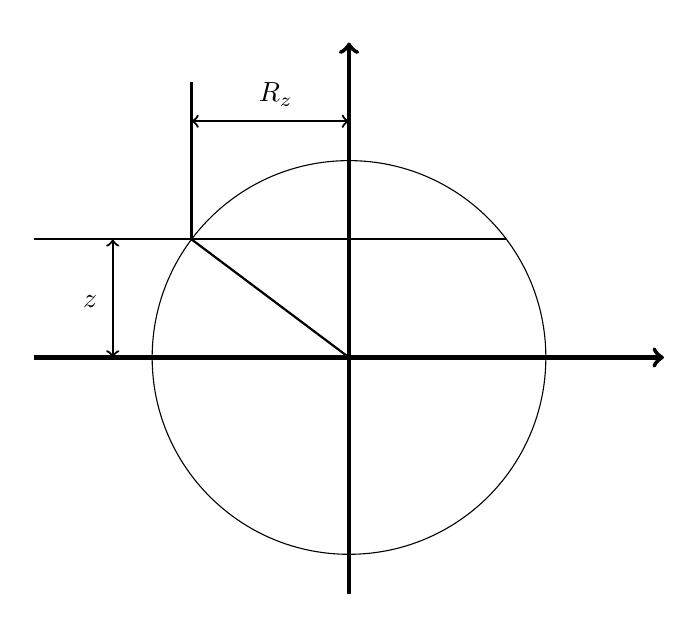
\begin{tikzpicture}
\draw (0, 0) circle (2.5);
\draw[ultra thick, ->] (-4, 0) -- (4, 0);
\draw[ultra thick, ->] (0, -3) -- (0, 4);
\draw[thick] (-4, 1.5) -- (2.0, 1.5);
\draw[thick] (0, 0) -- (-2.0, 1.5);
\draw[thick, <->] (-3, 0) -- (-3, 1.5)
  node[anchor=70, inner sep=20] {$z$};
\draw[thick] (-2.0, 1.5) -- (-2.0, 3.5);
\draw[thick, <->] (-2.0, 3) -- ( 0, 3)
  node[anchor=-20, inner sep=20] {$R_z$};
\end{tikzpicture}
\caption{\label{fig:vsphr}
Volume of a hypersphere ($D = 2$ case).}
\end{figure}

\item
The volume of the cross section is, therefore,
$$
A(z) = V_{D-1} \, R_z^{ D - 1 }.
$$

\item
The volume of the $D$-dimensional unit hypersphere
is given by
%
\begin{align}
  V_D
  &=
  \int_{-1}^1 A(z) \, dz
  \notag
  \\
  &=
  \int_{-1}^1 V_{D - 1} (1 - z^2)^{ \frac{ D - 1 } { 2 } } \, dz
  \notag
  \\
  &=
  V_{D - 1} \,
  \int_0^\pi \sin^D \theta \, d \theta
  \notag
  \\
  &=
  V_{D - 1} \,
  B\left(
     \frac{ D + 1 } { 2 }, \frac 1 2
   \right)
  \notag
  \\
  &=
  V_{D - 1} \,
  \frac{  \Gamma\left( \frac{ D + 1 } { 2 } \right)  }
       {  \Gamma\left( \frac{ D + 2 } { 2 } \right)  }
  \sqrt{ \pi }
  ,
  \label{eq:recur_VD}
\end{align}
%
where
$B(p, q) = \int_0^1 t^{p-1} \, (1-t)^{q-1} \, dt$
is the beta function.

\item
The solution of the recurrence relation, Eq. \eqref{eq:recur_VD},
is
\begin{align*}
  V_D
  =
  V_0 \,
  \frac{  \Gamma\left( \frac{ D + 1 } { 2 } \right)  }
       {  \Gamma\left( \frac{ D + 2 } { 2 } \right)  }
  \cdots
  \frac{  \Gamma\left( 1 \right)  }
       {  \Gamma\left( \frac{ 3 } { 2 } \right)  }
  \sqrt{ \pi }^D
  %
  =
  \frac{           \sqrt{ \pi }^D           }
       { \Gamma\left( \frac D 2 + 1 \right) }
  ,
\end{align*}
where we have used the initial condition
$V_1 = 2$ or $V_0 = 1$.

\item
In the close-packing lattice,
the maximal affordable radius is
half of the lattice constant.
Thus, the volume is
$$
V_D^{1/2}
=
V_D \,
\left( \frac 1 2 \right)^D
=
\frac{   \left( \sqrt \pi / 2 \right)^D   }
     { \Gamma\left( \frac D 2 + 1 \right) }
.
$$

\end{enumerate}






\section{Extensions}


We can extend the above analyses to two related quantities.
%
The first the coordination number,
or the number of nearest neighbors in a close-packing lattice.
%
The second is the distance between two next nearest neighbor vertices.
%
The latter may give an approximate cutoff distance
for the first coordination shell.


\section{Coordination number}


To compute the coordination number, $z_D$,
we note that each vertex, $P$,
in a $D$-dimensional close-packing lattice
lies in a layer of $(D-1)$-dimensional
close-packing lattice,
in which $P$ has $z_{D - 1}$ nearest neighbors.
%
Further, this $(D-1)$-dimensional layer
is sandwiched between two neighboring
$(D-1)$-dimensional close-packing layers.
%
In each of the neighboring layer,
vertex $P$ can find $D$ nearest neighbor vertices
to form a $D$-dimensional tetrahedron.
%
Therefore the coordination number, $z_D$
is given by
$$
z_D = z_{D - 1} + 2 \, D.
$$
%
The solution of the above recurrence relation,
with the initial condition $z_1 = 2$ is
$$
z_D = D \, (D + 1).
$$
%
This gives the coordination number
in a $D$-dimensional close-packing lattice.


\section{Distance between two next-nearest neighbors}


For the distance between two next-nearest neighbors,
we first note that the next nearest neighbor of $P$
necessarily lies in a neighboring $(D-1)$ layer
(otherwise the distance would be independent of the dimension, $D$).
%
An illustration is shown in Fig. \ref{fig:twolayers}.

\begin{figure}[h]
\centering
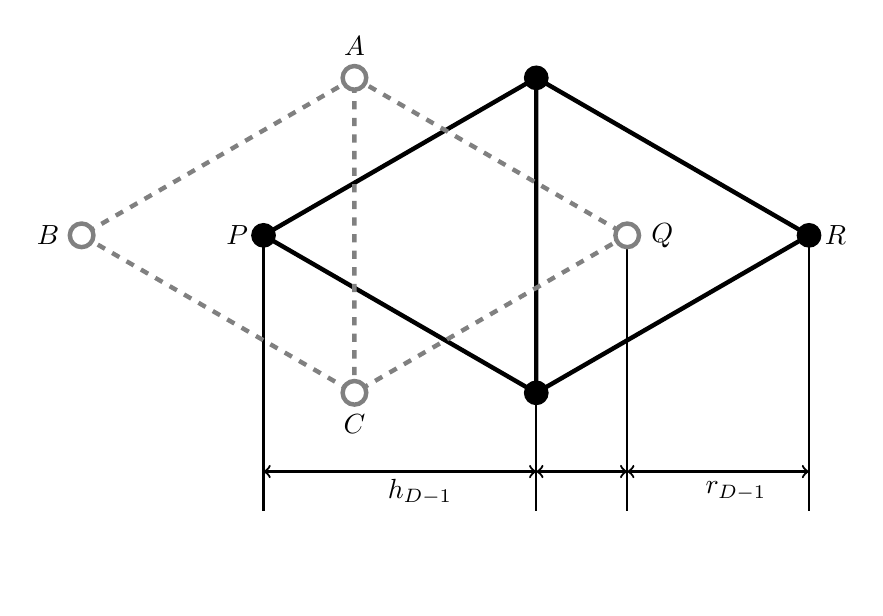
\begin{tikzpicture}
\draw[thick] ( 0.000, 0) -- ( 0.000, -3.5);
\draw[thick] (-3.464, 0) -- (-3.464, -3.5);
\draw[thick] ( 1.155, 0) -- ( 1.155, -3.5);
\draw[thick] ( 3.464, 0) -- ( 3.464, -3.5);
\draw[thick, <->] (-3.464, -3.0)   -- (0.0, -3.0)
    node[anchor=10, inner sep=30] {$h_{D-1}$};
\draw[thick, <->] (0.0, -3.0)   -- (1.155, -3.0)
    node[anchor=15, inner sep=0] {};
\draw[thick, <->] (1.155, -3.0) -- (3.464, -3.0)
    node[anchor=15, inner sep=15] {$r_{D-1}$};

% first layer
\draw[ultra thick] (0, 2.0) -- (-3.464, 0) -- (0, -2.0)
                -- (0, 2.0) -- ( 3.464, 0) -- (0, -2.0);
\draw[fill=black] ( 0,  2.0) circle (0.15);
\draw[fill=black] ( 0, -2.0) circle (0.15);
\draw[fill=black] ( 3.464, 0.0) circle (0.15); % R
\draw[fill=black] (-3.464, 0.0) circle (0.15); % P

\node at (-3.8, 0.0) {$P$};
\node at ( 3.8, 0.0) {$R$};

% second layer
\draw[ultra thick, gray, dashed]
                   (-2.309, 2.0) -- ( 1.155, 0.0) -- (-2.309, -2.0)
                -- (-2.309, 2.0) -- (-5.774, 0.0) -- (-2.309, -2.0);
\draw[ultra thick, gray, fill=white] (-2.309,  2.0) circle (0.15); % A
\draw[ultra thick, gray, fill=white] (-2.309, -2.0) circle (0.15); % C
\draw[ultra thick, gray, fill=white] ( 1.155, 0.0) circle (0.15); % Q
\draw[ultra thick, gray, fill=white] (-5.774, 0.0) circle (0.15); % B

\node at (-2.309,  2.4) {$A$};
\node at (-6.2,    0.0) {$B$};
\node at (-2.309, -2.4) {$C$};
\node at ( 1.6,    0.0) {$Q$};

%\draw[ultra thick] (-2.0, 0) -- (2.0, 0) -- (0.0, 3.464) -- cycle;
%\draw[ultra thick, dashed]
%   (-2.0, 0) -- (-4.0, 3.464) -- (0.0, 3.464);
%\draw[thick] (-2.0, 0)     -- (-2.0, -0.6)
%             ( 0.0, 3.464) -- ( 0.0, -0.6);
%\draw[thick, <->] (-2.0, -0.3) -- (0.0, -0.3)
%    node[anchor=20, inner sep=15] {$r_{D - 1}$};
%\draw[thick] ( 0.0, 3.464) -- ( 4.0, 3.464)
%             ( 0.0, 1.155) -- ( 3.0, 1.155)
%             ( 2.0, 0.0)   -- ( 4.0, 0.0);
%\draw[fill=white!80!black] ( 0, 1.155) circle (0.15);
\end{tikzpicture}
\caption{
\label{fig:twolayers}
Two neighboring $(D-1)$-dimensional layers
($D = 3$ here) from the top view.
%
The black and white dots represent
vertices from the first and second layers, respectively.
%
$A$, $B$ and $C$ nearest neighbors of $P$;
$Q$ is a next-nearest neighbor of $P$.
%
The horizontal distances are marked in the bottom.
}
\end{figure}

Here, $P$ and $Q$ are a pair of next nearest neighbors.
%
Since they lie in two different layers,
their distance, $d_{PQ}$, is given by
$$
d_{PQ}
=
\sqrt{
  d_{PQ, \bot}^2
  +
  d_{PQ, \parallel}^2
}.
$$
where
$d_{PQ, \bot}$
is the interlayer distance, $h_D$,
given by Eq. \eqref{eq:hD};
$d_{PQ, \parallel}$,
as the distance projection on the layer,
is given by
$$
d_{PQ, \parallel}
=
h_{D - 1} + ( h_{D - 1} - r_{D - 1} )
=
\frac{                   D + 1    }
     { \sqrt{ 2 \, D \, (D - 1) } }.
$$
Thus,
$$
d^\mathrm{\,nnn}_D
=
d_{PQ}
=
\sqrt{ \frac{ D + 1 } { D - 1 } }.
$$
This is the distance between two next-nearest neighbors
in a $D$-dimensional close-packing lattice.
%
Obviously, this formula is only good for $D > 1$.



\section{Table of values}

Below is a table of values.
\begin{table}[h]
\centering
\renewcommand{\arraystretch}{2.5}
\begin{tabular}{lllllll}
$D$     &   $V^{1/2}_D = \eta_D / \rho_D$
        &   $\eta^\mathrm{cp}_D$
        &   $z_D$
        &   $d^\mathrm{\,nnn}_D$ \\
\hline
$1$     &   $1$
        &   $1$
        &   $2$
        &   $2$
\\
$2$     &   $\dfrac{ \pi } { 4 } \approx 0.785$
        &   $\dfrac{ \pi } { 2 \, \sqrt 3 } \approx 0.907$
        &   $6$
        &   $\sqrt{3} \approx 1.732$
\\
$3$     &   $\dfrac{ \pi } { 6 } \approx 0.524$
        &   $\dfrac{ \pi } { 3 \, \sqrt 2 } \approx 0.740$
        &   $12$
        &   $\sqrt{2} \approx 1.414$
\\
$4$     &   $\dfrac{ \pi^2 } { 32 } \approx 0.308$
        &   $\dfrac{ \pi^2 } { 8 \, \sqrt{5} } \approx 0.552$
        &   $20$
        &   $\sqrt \frac 5 3 \approx 1.291$
\\
$5$     &   $\dfrac{ \pi^2 } { 60 } \approx 0.164$
        &   $\dfrac{ \pi^2 } { 15 \, \sqrt 3 } \approx 0.380$
        &   $30$
        &   $\sqrt \frac 3 2 \approx 1.225$
\\
$6$     &   $\dfrac{ \pi^3 } { 384 } \approx 0.0807$
        &   $\dfrac{ \pi^3 } { 48 \sqrt{7} } \approx 0.244$
        &   $42$
        &   $\sqrt \frac 7 5 \approx 1.183$
\\
$7$     &   $\dfrac{ \pi^3 } { 840 } \approx 0.0369$
        &   $\dfrac{ \pi^3 } { 210 } \approx 0.148$
        &   $56$
        &   $\sqrt \frac 4 3 \approx 1.155$
\\
$8$     &   $\dfrac{ \pi^4 } { 6144 } \approx 0.01585$
        &   $\dfrac{ \pi^4 } { 1152 } \approx 0.085$
        &   $72$
        &   $\sqrt \frac 9 7 \approx 1.134$
\\
$9$     &   $\dfrac{ \pi^4 } { 15120 } \approx 0.00644$
        &   $\dfrac{ \pi^4 } { 945 \, \sqrt 5 } \approx 0.046$
        &   $90$
        &   $\sqrt \frac 5 4 \approx 1.118$
\end{tabular}
\caption{
Volume of a unit-diameter hypersphere,
$V^{1/2}_D$,
close-packing fraction,
$\eta^\mathrm{cp}$,
coordination number,
$z_D$,
and
the distance between two next-nearest neighbors
in various dimensions.}
\end{table}

%The \textsc{Mathetmaica} code is
%\texttt{Table[{(pi/2)^{n/2}/sqrt{n+1}/Gamma[n/2+1], (pi*.5)^{n/2}/sqrt{n+1}/Gamma[n/2+1]}, {n,1,9}]}.




\end{document}
